%! TEX rootmain.tex

\chapter{Guitar}

The guitar is a plucked string instrument in which string vibration is transmitted through the bridge to a lightweight wooden soundboard and to the enclosed air volume of the body. Following the course outline, the discussion begins with the main parts of the instrument, then moves to the excitation mechanism (plucking), the description of the guitar as a system of coupled vibrators, the impact of structural modifications on vibrational properties, the modeling of plucked strings, the response to string forces, and finally sound radiation.

\section{Parts of the Guitar}

A classical guitar can be described in terms of a few functional subsystems: the string-bearing neck, the bridge region where forces are applied to the body, and the resonant box formed by top, back, and ribs. An exploded view highlights the main components: the head with tuning machines, the nut, the neck and fretboard, the body top with rosette and sound hole, the bridge and saddle, the side ribs, the back plate, and the tail block closing the enclosure. An exploded view of a classical guitar and its main components is shown in figure \ref{fig:guitar_exploded_view}.

\begin{figure}[!htb]
\centering
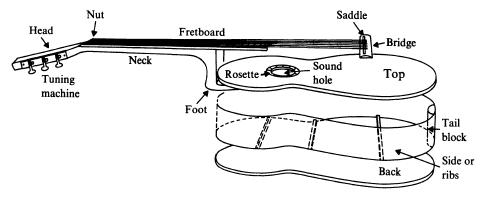
\includegraphics[width=0.85\linewidth]{00_Images/01_chapter/img59.jpg}
\caption{Exploded view of a classical guitar highlighting the main components}
\label{fig:guitar_exploded_view}
\end{figure}

Some construction features that are commonly specified are the following:

\begin{itemize}
    \item The instrument has six strings, about \SI{65}{\centi\meter} in length, tuned to \( E_2 \), \( A_2 \), \( D_3 \), \( G_3 \), \( B_3 \), and \( E_4 \), with fundamental frequencies
    \[
    f = \{\SI{82}{\hertz}, \SI{110}{\hertz}, \SI{147}{\hertz}, \SI{196}{\hertz}, \SI{247}{\hertz}, \SI{330}{\hertz}\}
    \]
    \item The top plate is usually cut from spruce or redwood, with thickness of about \SI{2.5}{\milli\meter}.
    \item The back plate is usually a hardwood, such as rosewood, mahogany, or maple, with thickness of about \SI{2.5}{\milli\meter}.
\end{itemize}

A key internal element of the soundboard is the bracing, namely a set of wooden strips glued to the inner side of the top plate. Bracing patterns alter the stiffness distribution of the soundboard and, as a consequence, strongly influence the vibrational behavior and the acoustic properties of the instrument. Several bracing layouts are commonly encountered or have been proposed over the years. Typical examples include traditional fan bracing, the Bouchet pattern (France), the Ramirez pattern (Spain), and crossed bracing, which uses intersecting braces to create an X-like reinforcement of the top plate. Representative bracing layouts are compared in figure \ref{fig:guitar_bracing_patterns}.

\begin{figure}[!htb]
\centering
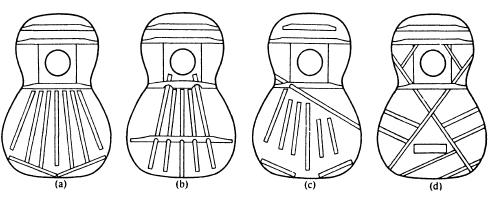
\includegraphics[width=0.95\linewidth]{00_Images/01_chapter/img77.jpg}
\caption{Examples of common soundboard bracing patterns for classical guitars}
\label{fig:guitar_bracing_patterns}
\end{figure}

\section{Excitation Mechanism in the Guitar: Plucking}

\subsection{Phases of the Plucking}

The excitation mechanism is crucial in plucked instruments because the first few milliseconds of the sound carry strong timbral cues: if this initial transient is removed, it becomes difficult to distinguish one instrument from another. Plucking can be described in terms of two main phases:

\begin{itemize}
    \item Stick phase: The string is displaced from its equilibrium position by an external force that can be idealized as concentrated at the plucking point \( x_0 \),
    \[
    F(x,t) = F_0\delta(x-x_0)
    \]
    As long as the applied force remains below a threshold \( F_{\mathrm{m}} \), the string stays stuck to the finger. In this phase a torsional component may also be present.
    \item Slip phase: When the restoring force reaches the threshold \( F_{\mathrm{m}} \), the string starts to slip under the finger. During slip, the finger or plectrum exerts a frictional force that introduces damping.
\end{itemize}

\subsection{Finger Articulation Model}

The finger can be modeled as a nonlinear spring with force-displacement relationship
\[
S(\xi)=
\begin{cases}
\dfrac{\sigma_1\xi}{\sigma_2-\xi} & \text{for } 0 \le \xi < \sigma_2 \\
\dfrac{\sigma_1\xi}{\sigma_2+\xi} & \text{for } -\sigma_2 < \xi < 0
\end{cases}
\]
This model captures an asymmetric, strongly nonlinear stiffness that increases rapidly as \( \xi \) approaches \( \pm\sigma_2 \), which is consistent with the limited range of finger articulation. The corresponding geometry and the nonlinear force-displacement characteristic are summarized in figure \ref{fig:finger_articulation_model}.

\begin{figure}[!htb]
\centering
\subfloat[]{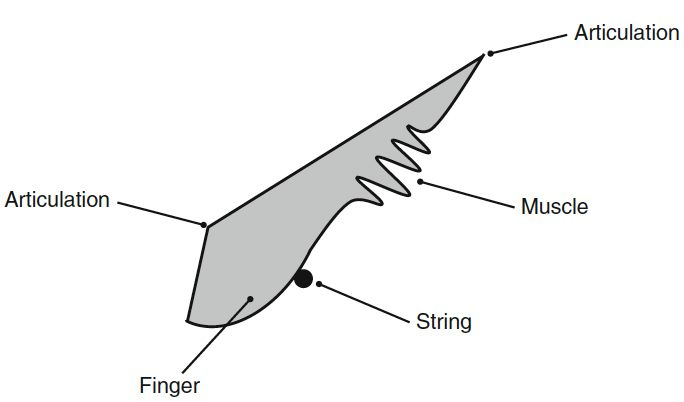
\includegraphics[width=0.45\linewidth]{00_Images/01_chapter/img127.jpg}}\hfill
\subfloat[]{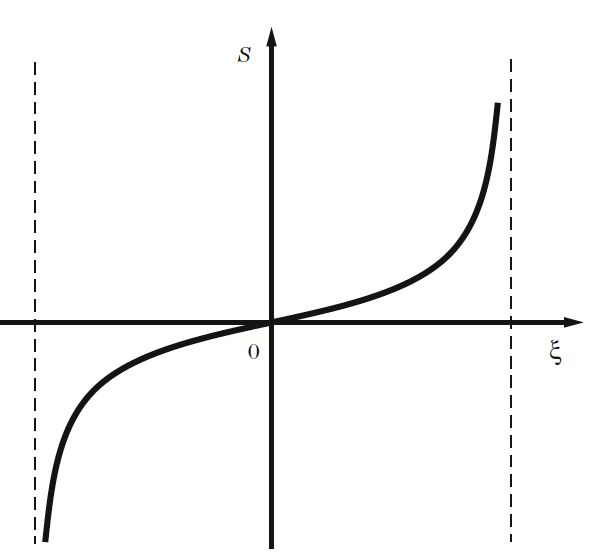
\includegraphics[width=0.45\linewidth]{00_Images/01_chapter/img129.jpg}}
\caption{Finger articulation model: schematic representation and nonlinear stiffness law}
\label{fig:finger_articulation_model}
\end{figure}

\subsection{Dynamic Friction Model of the Finger}

A dynamic description of the finger-string interaction considers different ingredients across the three stages of the motion.

\begin{itemize}
    \item During the stick phase: transversal motion of the string, rotation of the fingertip, torsional motion of the string, and the relative velocity between string and finger, which is ideally zero but may not be exactly so in practice.
    \item During the slip phase: the friction coefficient \( \mu \) depends on the relative velocity \( V_{\mathrm{rel}} \) between the string and the nail, according to
    \[
    \mu =
    \begin{cases}
    -\dfrac{\mu_S V_0 - \mu_d V_{\mathrm{rel}}}{V_{\mathrm{rel}} + V_0} & \text{for } V_{\mathrm{rel}} > 0  \\
    \dfrac{\mu_S V_0 - \mu_d V_{\mathrm{rel}}}{V_0 -    V_{\mathrm{rel}}} & \text{for } V_{\mathrm{rel}} < 0
    \end{cases}
    \]
    \item During free oscillations: the string motion is governed by transversal wave equations with two polarizations, perpendicular and parallel to the bridge, together with torsional dynamics.
\end{itemize}

A typical velocity-dependent friction law and a representative plucking-force time history are shown in figure \ref{fig:dynamic_friction_plucking_force}.

\begin{figure}[!htb]
\centering
\subfloat{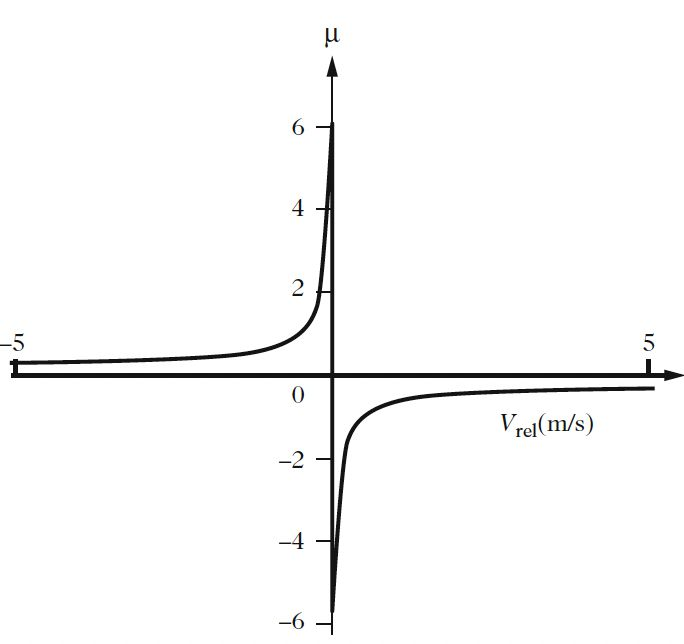
\includegraphics[width=0.45\linewidth]{00_Images/01_chapter/img151.jpg}}\hfill
\subfloat{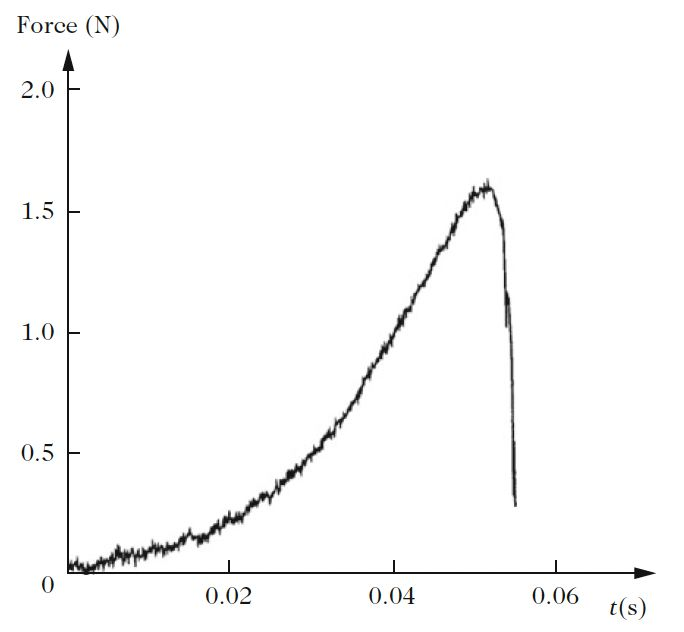
\includegraphics[width=0.45\linewidth]{00_Images/01_chapter/img153.jpg}}
\caption{Dynamic friction in plucking: friction coefficient versus relative velocity and an example force profile}
\label{fig:dynamic_friction_plucking_force}
\end{figure}

\section{The Guitar as a System of Coupled Vibrators}

\subsection{Sound Generation: Energy Flow in the Instrument}

Sound generation can be summarized as a chain of coupled subsystems. The strings mainly provide a driving force that sets the bridge region and the top plate into motion, and energy is then transferred to the enclosed air, the ribs, and the back. A simplified description of the main pathways is the following:

\begin{itemize}
    \item The strings put into vibration the bridge region and the top plate.
    \item Energy is transferred to the air cavity, ribs, and back plate.
    \item Sound is radiated efficiently by the top plate, the air cavity, and the back.
    \item At low frequency the top plate transmits energy to the back through both ribs and air cavity.
    \item At high frequency most of the sound is radiated by the top plate.
    \item At low frequency the bridge can be regarded as transparent, and it can be omitted from a minimal scheme.
\end{itemize}

A compact overview of the coupled subsystems involved in sound generation is shown in figure \ref{fig:guitar_energy_flow}.

\begin{figure}[!htb]
\centering
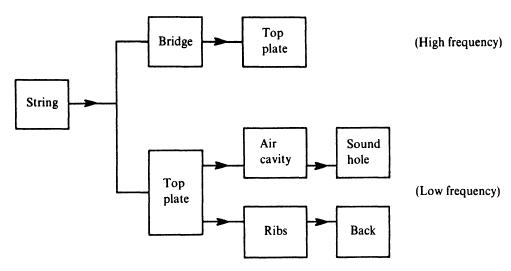
\includegraphics[width=0.9\linewidth]{00_Images/01_chapter/img170.jpg}
\caption{Energy flow and coupling pathways in the guitar body}
\label{fig:guitar_energy_flow}
\end{figure}

In what follows, a sequence of lumped-parameter models is introduced, with increasing complexity, in order to capture the low-frequency coupled behavior.

\subsection{Modeling by a Two-mass System}

If the motion of back and ribs is neglected, the guitar can be modeled as a two-degree-of-freedom vibrating system. The two subsystems are identified as follows:

\begin{itemize}
    \item The top plate, driven by the string force \( F(t) \), characterized by an effective mass \( m_p \) and stiffness \( K_p \).
    \item The Helmholtz resonator, represented by the mass of air \( m_h \) oscillating in the soundhole, while the enclosed air volume \( V \) provides the spring effect through compressibility.
\end{itemize}

An equivalent electrical circuit can be introduced, in which the analogous currents are volume velocities. The mechanical two-mass representation and the corresponding electrical analog are shown in figure \ref{fig:two_mass_electrical_analog}.

\begin{figure}[!htb]
\centering
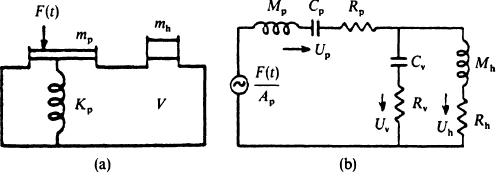
\includegraphics[width=0.95\linewidth]{00_Images/01_chapter/img189.jpg}
\caption{Two-mass guitar model and its electrical analog in terms of volume velocities}
\label{fig:two_mass_electrical_analog}
\end{figure}

\paragraph{Electrical analog and aymbols} In the electrical analog, the main quantities are expressed in terms of inertances and compliances. The symbols used are:

\begin{itemize}
    \item \( M_p = m_p/A_p^{2} \), inertance of the top plate.
    \item \( M_h = m_h/A_h^{2} \), inertance of the air in the soundhole.
    \item \( C_p = A_p^{2}/K_p \), compliance of the top plate.
    \item \( C_v = V/(\rho c^{2}) \), compliance of the enclosed air.
    \item \( U_p \), volume velocity of the top plate.
    \item \( U_h \), volume velocity of the air in the soundhole.
    \item \( U_v \), volume velocity associated with the air in the cavity.
    \item \( R_p \), losses (mechanical and radiative) associated with the top plate.
    \item \( R_h \), losses due to radiation from the soundhole.
    \item \( R_v \), losses associated with the enclosure.
\end{itemize}

\paragraph{Resonances and antiresonance} The coupled system exhibits two resonances with an antiresonance between them. Their qualitative interpretation can be summarized as follows:

\begin{itemize}
    \item At the lower resonance, the air flow through the soundhole is approximately in phase with the inward motion of the top plate, so that \( U_p \) and \( U_h \) are nearly in phase.
    \item At the upper resonance, air moves into the soundhole when the plate moves inward, leading to an out-of-phase relation between \( U_p \) and \( U_h \).
    \item The antiresonance corresponds to the Helmholtz resonance of the enclosure: \( U_v \) and \( U_h \) are equal and opposite, and consequently \( U_p \) reaches a minimum.
\end{itemize}

This circuit is able to capture the low-frequency response of a real guitar, for example when back plate and ribs are effectively immobilized. An example of measured low-frequency response consistent with the two-oscillator description is shown in figure \ref{fig:low_frequency_response_example}.

\begin{figure}[!htb]
\centering
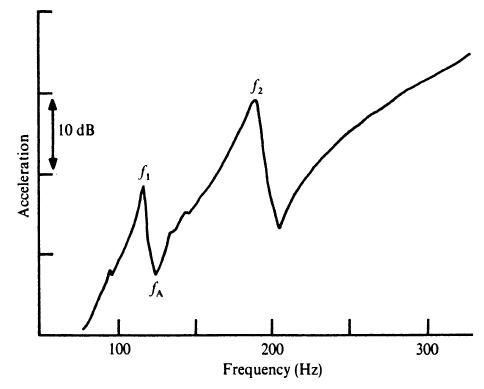
\includegraphics[width=0.7\linewidth]{00_Images/01_chapter/img204.jpg}
\caption{Example of low-frequency response captured by a minimal coupled model}
\label{fig:low_frequency_response_example}
\end{figure}

\subsection{Coupling at Low Frequencies between the Top Plate and the Cavity}

At low frequencies the interaction between the first (lowest) mode of the soundboard and the lowest acoustic mode of the cavity can be captured by a two-degree-of-freedom model. The soundboard is represented by a rigid body with mass \( m_p \), area \( A_p \), and intrinsic stiffness \( k_p \), subject to the vertical string force \( F \). Its vertical displacement is denoted by \( \xi_p \), interpreted as a mean displacement associated with the first structural mode. The soundbox is represented as a Helmholtz resonator with one moving wall. The inertial part is the mass of air \( m_h \) oscillating through holes of total area \( A_h \), with displacement \( \xi_h \). The volume change in the cavity is
\[
\Delta V = A_p \xi_p + A_h \xi_h
\]
Air compressibility produces a pressure change
\[
\Delta p = -\rho c^{2}\frac{\Delta V}{V} = -\mu\left(A_p \xi_p + A_h \xi_h\right)
\]
where
\[
\mu = \frac{\rho c^{2}}{V}
\]
Losses are modeled through a diagonal damping matrix with constants \( R_p \) for the plate and \( R_h \) for the soundbox, assumed approximately constant with frequency. The equations of motion can be written in matrix form as
\[
\begin{bmatrix}
m_p & 0 \\
0   & m_h
\end{bmatrix}
\begin{bmatrix}
\ddot{\xi}_p \\
\ddot{\xi}_h
\end{bmatrix}
+
\begin{bmatrix}
R_p & 0 \\
0   & R_h
\end{bmatrix}
\begin{bmatrix}
\dot{\xi}_p \\
\dot{\xi}_h
\end{bmatrix}
+
\begin{bmatrix}
k_p + \mu A_p^{2} & \mu A_h A_p \\
\mu A_h A_p       & \mu A_h^{2}
\end{bmatrix}
\begin{bmatrix}
\xi_p \\
\xi_h
\end{bmatrix}
=
\begin{bmatrix}
F \\
0
\end{bmatrix}
\]
Three limiting cases are useful to interpret the parameters:

\begin{itemize}
    \item With a closed hole, \( A_h = 0 \), the box acts on the board as an added stiffness \( \mu A_p^{2} \), and the undamped eigenfrequency becomes
    \[
    \omega_p = \sqrt{\frac{k_p + \mu A_p^{2}}{m_p}}
    \]
    \item If the board stiffness is negligible, the corresponding angular frequency becomes
    \[
    \omega_a = \sqrt{\frac{\mu A_p^{2}}{m_p}}
    \]
    \item If the board is held fixed, \( \xi_p = 0 \), the soundbox reduces to a Helmholtz resonator with
    \[
    \omega_h = \sqrt{\frac{\mu A_h^{2}}{m_h}}
    \]
\end{itemize}

The eigenfrequencies of the associated conservative coupled system satisfy
\[
\det\left(K - \omega^{2}M\right)=0
\]
which leads to
\[
\left(\omega_p^{2}-\omega^{2}\right)\left(\omega_h^{2}-\omega^{2}\right)-\omega_{ph}^{4}=0
\]
with
\[
\omega_{ph}^{4}=\omega_a^{2}\omega_h^{2}
\]
With typical guitar values, one finds for instance \( f_h \approx \SI{100}{\hertz} \) and \( f_a \approx \SI{200}{\hertz} \), leading to two split coupled resonances around \( f_1 \approx \SI{86}{\hertz} \) and \( f_2 \approx \SI{206.5}{\hertz} \). In this interpretation, \( f_1 \) is the Helmholtz resonance with non-rigid walls and \( f_2 \) is associated with the first top-plate mode \( T_1 \). The coupling therefore separates the original uncoupled frequencies, and it also holds that
\[
\omega_1^{2}+\omega_2^{2}=\omega_p^{2}+\omega_h^{2}
\]

\subsection{The Three-mass Model}

If the back plate is allowed to move, a three-oscillator model is obtained. In this case the ribs are assumed immobilized, and the coupling between top and back is enabled primarily by the air in the cavity. In the electrical analog, the back plate is represented by an inertance \( M_b \), a compliance \( C_b \), a loss \( R_b \), and a corresponding volume velocity \( U_b \). The response of this system is characterized by three resonances \( f_1 \), \( f_2 \), and \( f_3 \), and by two antiresonances \( f_A \) and \( f_B \). The three-oscillator electrical analog and its characteristic resonance/antiresonance pattern are shown in figure \ref{fig:three_mass_model}.

\begin{figure}[!htb]
\centering
\subfloat{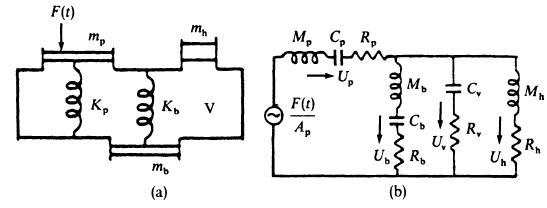
\includegraphics[width=0.58\linewidth]{00_Images/01_chapter/img300.jpg}}\hfill
\subfloat{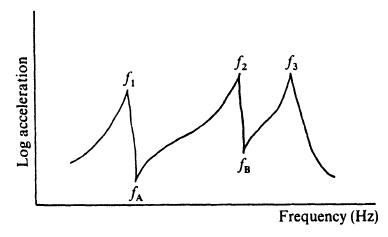
\includegraphics[width=0.38\linewidth]{00_Images/01_chapter/img319.jpg}}
\caption{Three-mass model: electrical analog and typical low-frequency response}
\label{fig:three_mass_model}
\end{figure}

\section{Structural Modifications of the Instrument}

Examples of construction differences and their impact on the vibrational/acoustical balance are illustrated in figure \ref{fig:structural_modifications_example}.

\begin{figure}[!htb]
\centering
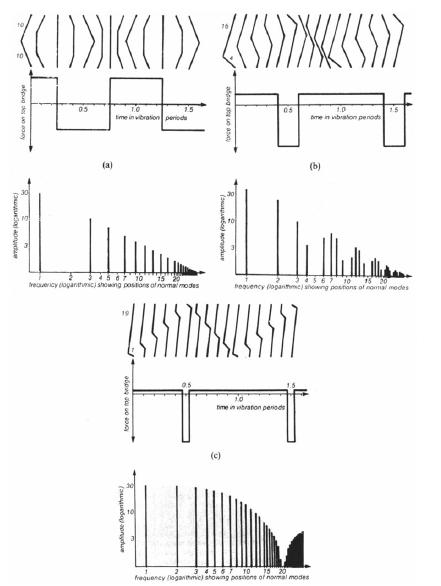
\includegraphics[width=0.7\linewidth]{00_Images/01_chapter/img481.jpg}
\caption{Illustrative example of structural modifications and associated spectral consequences}
\label{fig:structural_modifications_example}
\end{figure}

\subsection{Sensitivity of Eigenvalues to Structural Parameters}

To study how construction changes affect the low-frequency coupled behavior, it is convenient to consider the undamped generalized eigenvalue problem
\[
K \phi = \lambda M \phi
\]
where \( K \) is the stiffness matrix, \( M \) is the mass matrix, \( \phi \) is an eigenvector, and the eigenvalue is related to the angular eigenfrequency by
\[
\lambda = \omega^{2}
\]
Let \( a \) be a physical or geometrical parameter, such as a mass, a cavity volume, or the area of an opening. Differentiating the eigenvalue equation with respect to \( a \) gives
\[
\frac{\partial K}{\partial a}\phi + K\frac{\partial \phi}{\partial a}
=
\frac{\partial \lambda}{\partial a}M\phi + \lambda \frac{\partial M}{\partial a}\phi + \lambda M\frac{\partial \phi}{\partial a}
\]
From this relation, one obtains the sensitivity of the eigenvalues
\[
\frac{\partial \lambda}{\partial a}
=
\frac{\phi^{T}\dfrac{\partial K}{\partial a}\phi - \lambda \phi^{T}\dfrac{\partial M}{\partial a}\phi}{\phi^{T}M\phi}
\]
This expression links the frequency shifts directly to how the matrices \( K \) and \( M \) depend on the chosen parameter.

\subsection{Effect of Soundboard Mass}

Consider the two-degree-of-freedom model introduced earlier, with soundboard mass \( m_p \) and air mass in the soundhole \( m_h \). Setting \( a=m_p \), only the mass matrix is affected, and
\[
\frac{\partial M}{\partial m_p}
=
\begin{bmatrix}
1 & 0 \\
0 & 0
\end{bmatrix}
\]
If the mode shapes are assumed not to change significantly with a small modification of \( m_p \), the \( i \)-th eigenvalue sensitivity can be written as
\[
\frac{\partial \lambda_i}{\partial m_p}
=
-\frac{\lambda_i \phi_{i1}^{2}}{m_p\phi_{i1}^{2}+m_h\phi_{i2}^{2}}
\]
An increase of soundboard mass therefore reduces the eigenvalues and lowers the corresponding eigenfrequencies.

\subsection{Effect of Cavity Volume}

Setting \( a=V \), only the stiffness matrix changes through the cavity compliance. With \( \mu=\rho c^{2}/V \), one obtains
\[
\frac{\partial K}{\partial V}
=
-\frac{c^{2}\rho}{V^{2}}
\begin{bmatrix}
A_p^{2} & A_hA_p \\
A_hA_p  & A_h^{2}
\end{bmatrix}
\]
and the sensitivity becomes
\[
\frac{\partial \lambda_i}{\partial V}
=
-\frac{\dfrac{c^{2}\rho}{V^{2}}\left(A_p^{2}\phi_{i1}^{2}+2A_pA_h\phi_{i1}\phi_{i2}+A_h^{2}\phi_{i2}^{2}\right)}{m_p\phi_{i1}^{2}+m_h\phi_{i2}^{2}}
\]
An increase of the soundbox volume lowers the eigenfrequencies, which is consistent with the historical trend toward larger-bodied instruments.

\subsection{Effect of Soundhole Area and Thickness}

The mass of air in the opening can be written as
\[
m_h = \rho h A_h
\]
where \( h \) is an effective thickness of the opening. A change in opening area \( A_h \) affects both stiffness and mass:
\[
\frac{\partial K}{\partial A_h}
=
\mu
\begin{bmatrix}
0   & A_p \\
A_p & 2A_h
\end{bmatrix}
\quad
\frac{\partial M}{\partial A_h}
=
\begin{bmatrix}
0 & 0 \\
0 & \rho h
\end{bmatrix}
\]
leading to
\[
\frac{\partial \lambda_i}{\partial A_h}
=
\frac{2\mu\left(A_p\phi_{i1}\phi_{i2}+A_h\phi_{i2}^{2}\right)-\lambda_i\rho h\phi_{i2}^{2}}{m_p\phi_{i1}^{2}+m_h\phi_{i2}^{2}}
\]
In this simplified setting, increasing the total area of the openings tends to increase the eigenfrequencies, while increasing the effective thickness \( h \) has the opposite effect through the added air mass.

\subsection{Effect of Soundboard Thickness and Bracing}

Makers commonly modify the overall stiffness of the soundboard either by varying its thickness or by adding stiffeners (bracing), or both. If the thickness \( e \) is varied, the mass scales approximately in proportion to \( e \), whereas the bending stiffness scales approximately as \( e^{3} \), so stiffness changes can dominate. For simplicity, one may isolate the effect of an effective plate stiffness \( k_p \), keeping \( m_p \) fixed. With \( a=k_p \), the sensitivity becomes
\[
\frac{\partial \lambda_i}{\partial k_p}
=
\frac{\phi_{i1}^{2}}{m_p\phi_{i1}^{2}+m_h\phi_{i2}^{2}}
\]
An increase of \( k_p \) raises the eigenfrequencies, while a decrease of thickness, which typically reduces effective stiffness, lowers them.

\section{Modeling of Plucked Strings}

\subsection{Force Exerted by the Strings}

When a string is plucked, the tension \( T \) applies a force to the bridge that can be decomposed into a component normal to the top plate and a component parallel to it. Let \( \theta \) be the plucking angle. The two components are
\[
T\sin\theta \quad \text{(normal to the plate)}, \qquad T\cos\theta \quad \text{(parallel to the plate)}
\]
During the vibration cycle the string length changes slightly, which induces a time-varying tension. If \( A \) is the string cross-section, \( E \) its Young's modulus, and \( L_0 \) the nominal length, the tension can be written as
\[
T = T_0 + \Delta T = T_0 + \frac{EA}{L_0}\Delta L
\]
For small \( \theta \), the transverse and longitudinal force components at the bridge become
\[
F_T = (T_0+\Delta T)\sin\theta
\]
\[
F_L = (T_0+\Delta T)\cos\theta \simeq T_0+\Delta T = T_0 + \frac{EA}{L_0}\Delta L
\]
Consider a string displaced by a distance \( d \) at a point located at \( \beta L_0 \) from the bridge and then released. The two string segments form angles \( \theta_1 \) and \( \theta_2 \) with
\[
\sin\theta_1 \simeq \frac{d}{\beta L_0}
\qquad
\sin\theta_2 = \frac{d}{(1-\beta)L_0}
\]
The longitudinal force component \( F_L \) has a slight time dependence due to the change in string length during the cycle. The maximum elongation can be estimated from the two-segment geometry as
\[
\Delta L_{\max}
=
\sqrt{\beta^{2}L_{0}^{2}+d^{2}}
+
\sqrt{(1-\beta)^{2}L_{0}^{2}+d^{2}}
-
L_{0}
\]
A minimum elongation is reached when the bend is located at \( 2\beta L_0 \), leading to
\[
\Delta L_{\min}
=
\sqrt{4\beta^{2}L_{0}^{2}+\frac{(1-2\beta)^{2}}{(1-\beta)^{2}}d^{2}}
+
\sqrt{(1-2\beta)^{2}L_{0}^{2}+\frac{(1-2\beta)^{2}}{(1-\beta)^{2}}d^{2}}
-
L_{0}
\]
Some qualitative consequences follow from the previous relations:

\begin{itemize}
    \item For nylon strings and small \( d \), the transverse component can largely dominate the longitudinal one, \( F_T \gg F_L \).
    \item The coupling between transverse string motion and top-plate motion is typically more effective than the coupling associated with the parallel component.
    \item Increasing \( d \) increases the relevance of the component parallel to the plate.
    \item For steel strings the difference between \( F_L \) and \( F_T \) is generally less pronounced.
\end{itemize}

The plucking position also matters. As \( \beta \) decreases, both transverse and longitudinal forces increase, while at the same time a larger applied effort is required to reach the same deflection \( d \). This is reflected in the waveform and in the corresponding spectrum, which change noticeably when the pluck is moved closer to the bridge. Typical changes in waveform and spectrum as the plucking point approaches the bridge are shown in figure \ref{fig:pluck_position_waveform_spectrum}.

\begin{figure}[!htb]
\centering
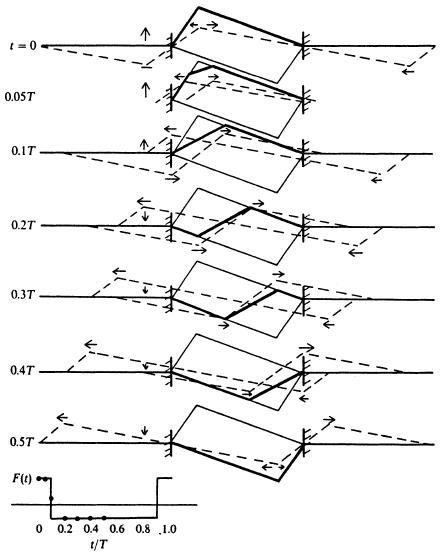
\includegraphics[width=0.7\linewidth]{00_Images/01_chapter/img495.jpg}
\caption{Influence of plucking position on time waveform and corresponding spectrum}
\label{fig:pluck_position_waveform_spectrum}
\end{figure}

\subsection{Modeling}

In the coupled models introduced earlier, attention was focused on transfer functions, without explicitly describing the excitation. For a plucked string, the initial condition produced by the pluck strongly shapes the waveform and therefore the radiated sound. A standard description of string motion is based on the superposition of two traveling waves propagating in opposite directions and reflecting at the terminations. Under the assumption that, during autonomous vibration, the string can be regarded as a linear time-invariant system, this leads to efficient computational models. A widely used representation is the bidirectional digital waveguide: two delay lines implement the propagation in the two directions, while reflection filters \( R_f(z) \) and \( R_b(z) \) account for phase inversion and frequency-dependent losses at the terminations. In this view, input and output signals may represent different wave variables, such as displacement, velocity, acceleration, or slope. Choosing acceleration as the wave variable is convenient, because an idealized pluck can be treated as an impulse-like excitation. For sound synthesis, it is often advantageous to commute propagation, losses, and dispersion into a single delay-loop structure. In this simplified single delay-loop model, the effects of losses and dispersion are lumped into a loop filter \( H_l(z) \). A particularly simple special case uses a two-point averaging loop filter and random initial conditions in the delay line, yielding the Karplus-Strong algorithm. This extreme simplification is computationally efficient but generally insufficient for high-quality synthesis or detailed physical interpretation. To connect the bidirectional waveguide description to an efficient single-loop form while preserving excitation and observation positions, it is useful to derive an equivalent linear transfer function for a given output, such as the transverse force at the bridge. In the Laplace domain, an equivalent single excitation at point \( E_1 \) can be introduced as
\[
X_{E_1,\mathrm{eq}}(s)
=
\frac{1}{2}\left[1+H_{E_2,E_1}(s)\right]X(s)
=
H_E(s)X(s)
\]
The bridge output of interest is the transverse force \( F(s) \), which can be related to the bridge impedance \( Z(s) \) and to the difference of the counter-propagating velocity components. Using accelerations \( A_1(s) \) and \( A_2(s) \),
\[
F(s)=Z(s)\frac{A_1(s)-A_2(s)}{s}
\]
If the backward-traveling component is expressed through a reflection \( R_b(s) \), this becomes
\[
F(s)=Z(s)\frac{\left[1-R_b(s)\right]A_1(s)}{s}=H_B(s)A_1(s)
\]
The acceleration at the bridge satisfies a recursion of the form
\[
A_1(s)=H_{E_1,R_1}(s)X_{E_1,\mathrm{eq}}(s)+H_{\mathrm{loop}}(s)A_1(s)
\]
with a loop transfer function
\[
H_{\mathrm{loop}}(s)=R_b(s)H_{R_2,E_2}(s)H_{E_2,E_1}(s)H_{E_1,R_1}(s)
\]
Solving for \( A_1(s) \) yields
\[
A_1(s)=H_{E_1,R_1}(s)\frac{1}{1-H_{\mathrm{loop}}(s)}X_{E_1,\mathrm{eq}}(s)
=
H_{E_1,R_1}(s)S(s)X_{E_1,\mathrm{eq}}(s)
\]
where \( S(s) \) represents the recursion around the loop. The overall transfer function from excitation to bridge force is then obtained by cascading the equivalent excitation, propagation, loop recursion, bridge coupling, and integration. A perceptually equivalent block diagram can be constructed by grouping the effects of excitation position, bridge coupling, and the integrator into a small set of filters around a delay-loop. In this interpretation, excitation position produces a comb-filter-like effect on the harmonic amplitudes, which is stronger as the pluck is moved away from the midpoint.

\subsection{Modeling of High-frequency Resonances}

The lumped analogs introduced for the body capture the low-frequency coupled behavior well, but they become insufficient at higher frequencies. To extend the validity, the body response can be analyzed in the frequency domain and each significant resonance can be rendered by a separate damped oscillator. Low-frequency oscillators retain a clear physical interpretation from the coupled models, while higher-frequency resonances are introduced by fitting the measured or computed frequency response.

\subsection{Coupling of Different Components}

A complete model can be assembled by coupling the string model to an electrical analog of the guitar body. In this representation, a resonant branch associated with the top plate is combined with elements representing the soundbox resonance and additional losses. The resulting network can reproduce both magnitude and phase of the body frequency response over a wider band when parameters are chosen consistently with measurements. A representative electrical analog for the guitar body used in coupled simulations is shown in figure \ref{fig:complete_body_model} and an example of agreement in both magnitude and phase for the body frequency response is shown in figure \ref{fig:body_frf_mag_phase}. The integration of the string model with the body analog is summarized in figure \ref{fig:string_body_integration}.

\subsection{Waveforms and Spectrograms}

Once string and body models are integrated, time-domain signals such as bridge velocity and force can be synthesized and compared with recorded quantities. Waveforms and corresponding spectrograms provide a compact way to verify whether the temporal evolution and the spectral envelope produced by the model are consistent with the measured excitation force and the recorded sound. A representative set of waveforms and the corresponding spectrograms is shown in figure \ref{fig:waveforms_spectrograms}.

\begin{figure}[!htb]
\centering
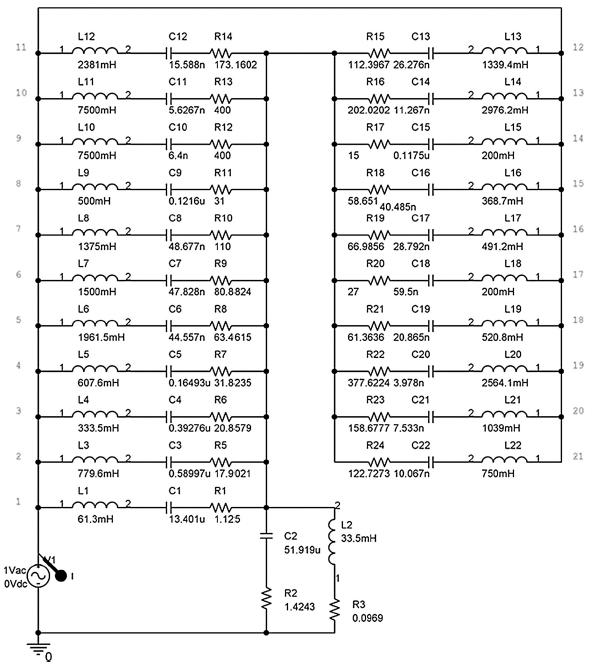
\includegraphics[width=0.8\linewidth]{00_Images/01_chapter/img554.jpg}
\caption{Electrical analog of the guitar body for broadband modeling}
\label{fig:complete_body_model}
\end{figure}

\begin{figure}[!htb]
\centering
\subfloat{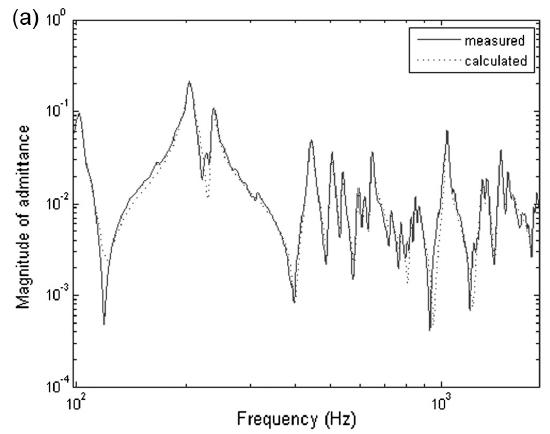
\includegraphics[width=0.45\linewidth]{00_Images/01_chapter/img568.jpg}}\hfill
\subfloat{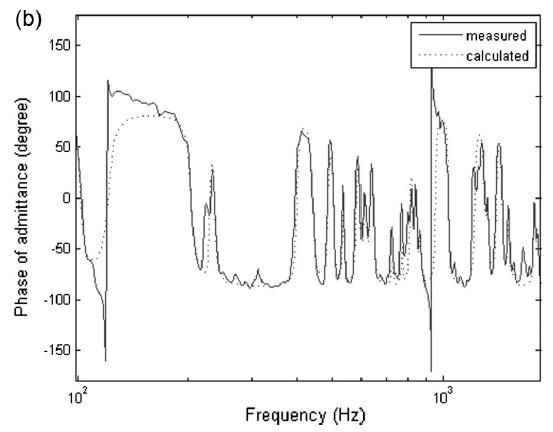
\includegraphics[width=0.45\linewidth]{00_Images/01_chapter/img578.jpg}}
\caption{Body frequency response function: magnitude and phase comparison}
\label{fig:body_frf_mag_phase}
\end{figure}

\begin{figure}[!htb]
\centering
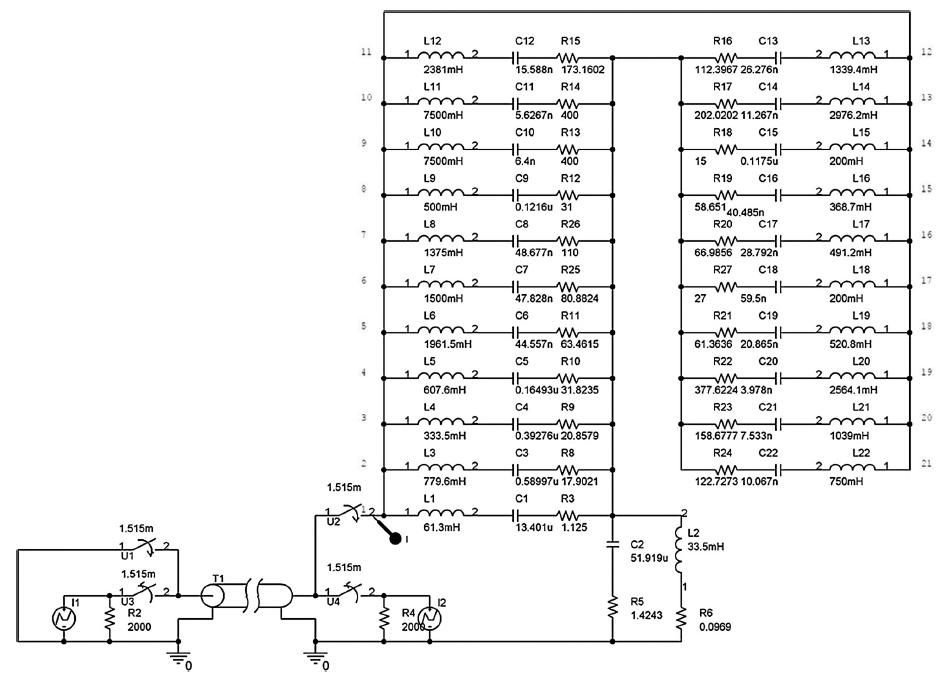
\includegraphics[width=0.7\linewidth]{00_Images/01_chapter/img592.jpg}
\caption{Integration of string and body models within a unified network representation}
\label{fig:string_body_integration}
\end{figure}

\begin{figure}[!htb]
\centering
\subfloat{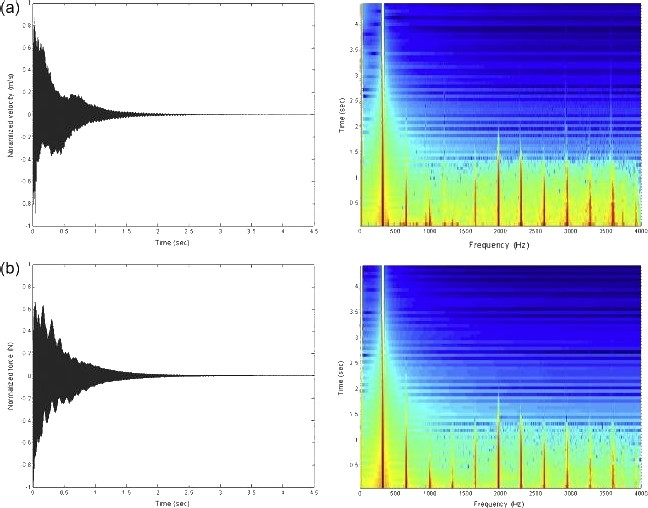
\includegraphics[width=0.45\linewidth]{00_Images/01_chapter/img606_1.jpg}}\hfill
\subfloat{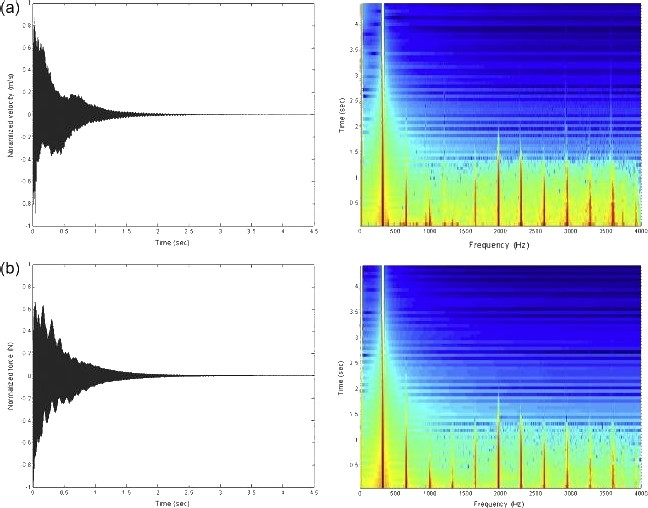
\includegraphics[width=0.45\linewidth]{00_Images/01_chapter/img606_1.jpg}}
\caption{Simulated or measured waveforms and corresponding spectrograms for model validation}
\label{fig:waveforms_spectrograms}
\end{figure}

\section{Response to String Forces}

The string action at the bridge can be decomposed into components that are parallel and orthogonal with respect to the bridge line. These components couple differently to the low-order vibration shapes of the soundboard. The main qualitative effects can be summarized as follows:

\begin{itemize}
    \item The force component parallel to the bridge is typically smaller in magnitude, but it promotes a rocking motion of the bridge, especially when the excitation is applied on one side of the bridge.
    \item The soundboard mode that is most efficiently excited by the horizontal, bridge-parallel action is the \( (1,0) \) mode.
    \item A force component orthogonal to the bridge can strongly excite the fundamental \( (0,0) \) resonance.
    \item If the orthogonal component is applied preferentially toward the treble or bass side, it can also excite the \( (1,0) \) mode.
\end{itemize}

\paragraph{Evidence from holographic interferometry} The different coupling mechanisms can be visualized through holographic interferograms of the top plate under controlled static actions. Distinct deformation patterns are observed when applying a lateral force parallel to the bridge, a force perpendicular to the bridge, a longitudinal force, or a twisting torque, confirming that the direction and point of application of the string-induced loading select different families of soundboard motion. Representative holographic interferograms illustrating the dependence on loading direction are shown in figure \ref{fig:holographic_interferograms}.

\begin{figure}[!htb]
\centering
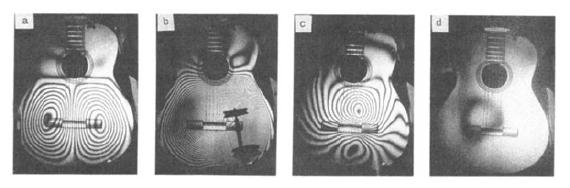
\includegraphics[width=0.8\linewidth]{00_Images/01_chapter/img622.jpg}
\caption{Holographic interferograms of the soundboard under different static actions at the bridge}
\label{fig:holographic_interferograms}
\end{figure}

\paragraph{Compound decay in normal plucking} In normal playing, the pluck direction is neither purely parallel nor purely orthogonal to the bridge, so both components are present at once. The orthogonal component tends to excite modes that are strong but decay rapidly, while the parallel component activates modes that are weaker but decay more slowly. As a result, the observed vibration envelope often shows a compound decay, with a fast initial reduction followed by a longer-lasting tail. An example of compound decay resulting from the coexistence of fast and slow modal components is shown in figure \ref{fig:compound_decay}.

\begin{figure}[!htb]
\centering
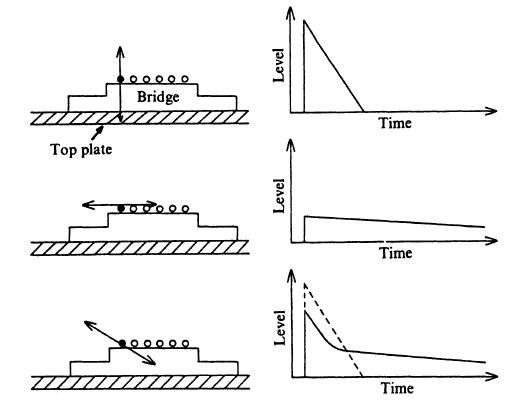
\includegraphics[width=0.6\linewidth]{00_Images/01_chapter/img636.jpg}
\caption{Example of compound decay envelope in normal plucking}
\label{fig:compound_decay}
\end{figure}

\section{Sound Radiation}

Sound radiation from the guitar is the result of a complex superposition of the radiation contributions associated with many structural and acoustic modes. Some low-frequency modes can radiate efficiently even when the instrument is driven well above their natural frequency, producing a smoothing effect on the resulting spectrum.

\paragraph{Mechanical response and radiated spectrum} A representative comparison can be made by considering a Martin D-28 guitar driven by a sinusoidal force of \SI{0.15}{\newton} applied at the treble side of the bridge, and observing the sound spectrum at \SI{1}{\meter} in front of the instrument. The measured acceleration level at the driving point highlights the mechanical resonances, while the radiated sound spectrum follows the overall trend but does not replicate it one-to-one, because radiation efficiency varies with frequency and mode shape. A representative comparison between mechanical response at the driving point and the radiated sound spectrum is shown in figure \ref{fig:mech_vs_radiated_spectrum}.

\begin{figure}[!htb]
\centering
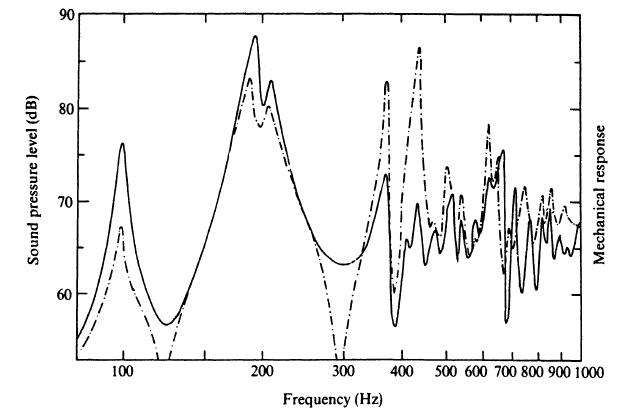
\includegraphics[width=0.45\linewidth]{00_Images/01_chapter/img654.jpg}
\caption{Driving-point mechanical response and radiated sound spectrum under sinusoidal forcing}
\label{fig:mech_vs_radiated_spectrum}
\end{figure}

\paragraph{Radiation patterns at resonances} Radiation directivity changes significantly across resonances. At lower frequencies, the patterns tend to be comparatively smooth, whereas at higher resonances the angular distribution becomes more structured, with multiple lobes and nulls. For instance, radiation patterns reported around \SI{102}{\hertz}, \SI{204}{\hertz}, \SI{376}{\hertz}, and \SI{436}{\hertz} show an evolution from simpler to more complex directivity shapes as frequency increases. Examples of measured radiation directivity at selected resonances are shown in figure \ref{fig:radiation_patterns_resonances}.

\begin{figure}[!htb]
\centering
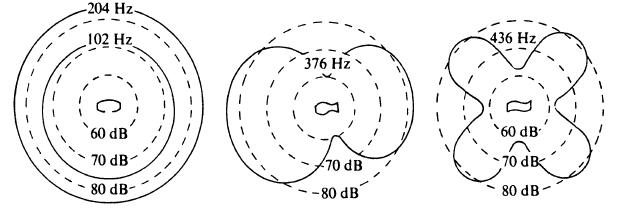
\includegraphics[width=0.7\linewidth]{00_Images/01_chapter/img668.jpg}
\caption{Radiation patterns at selected resonances illustrating the evolution of directivity with frequency}
\label{fig:radiation_patterns_resonances}
\end{figure}
